\documentclass{beamer}
%\documentclass[draft]{beamer}
%\documentclass[handout]{beamer}


\mode<handout>
{
  \usepackage{pgfpages}
  \pgfpagesuselayout{4 on 1}[a4paper,border shrink=3mm,landscape]
  \usetheme{Madrid}
  \usecolortheme{seagull}
}

\mode<beamer>
{
  \usetheme{Madrid}
  \setbeamercovered{transparent}
}


\usepackage[english]{babel}
\usepackage[utf8]{inputenc}

\usepackage{times}


\title{The Dynare Preprocessor}

\author[S. Villemot]{Sébastien Villemot}

\institute{CEPREMAP}

\date{October 19, 2007}

\AtBeginSection[]
{
  \begin{frame}{Outline}
    \tableofcontents[currentsection]
  \end{frame}
}

\begin{document}

\begin{frame}
  \titlepage
\end{frame}

\begin{frame}
  \frametitle{General overview}
  \begin{center}
    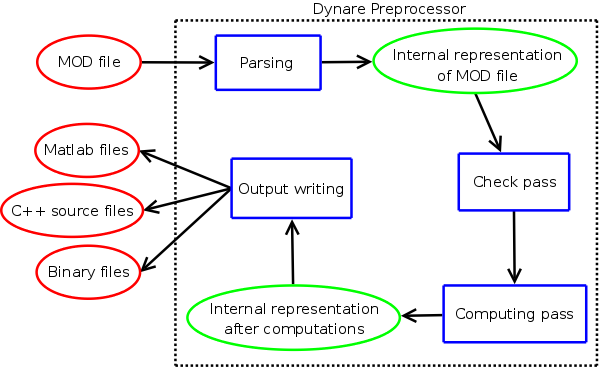
\includegraphics[width=11cm]{overview.png}
  \end{center}
\end{frame}

\begin{frame}{Outline}
  \tableofcontents
\end{frame}

\section{Parsing}

\begin{frame}
\frametitle{Parsing overview}
\begin{itemize}
\item Parsing is the action of transforming an input text (a \texttt{mod} file in our case) into a data structure suitable for computation
\item The parser consists of three components:
  \begin{itemize}
  \item the \alert{lexical analyzer}, which recognizes the ``words'' of the \texttt{mod} file (analog to the \textit{vocabulary} of a language)
  \item the \alert{syntax analyzer}, which recognizes the ``sentences'' of the \texttt{mod} file (analog to the \textit{grammar} of a language)
  \item the \alert{parsing driver}, which coordinates the whole process and constructs the data structure using the results of the lexical and syntax analyses
  \end{itemize}
\end{itemize}
\end{frame}

\begin{frame}
\frametitle{Lexical analysis}
\begin{itemize}
\item The lexical analyzer recognizes the ``words'' (or \alert{lexemes}) of the language
\item Lexical analyzer is described in \texttt{DynareFlex.ll}. This file is transformed into C++ source code by the program \texttt{flex}
\item This file gives the list of the known lexemes (described by regular expressions), and gives the associated \alert{token} for each of them
\item For punctuation (semicolon, parentheses, ...), operators (+, -, ...) or fixed keywords (\textit{e.g.} \texttt{model}, \texttt{varexo}, ...), the token is simply an integer uniquely identifying the lexeme
\item For variable names or numbers, the token also contains the associated string for further processing
%\item \textit{Note:} the list of tokens can be found at the beginning of \texttt{DynareBison.yy}
\item When invoked, the lexical analyzer reads the next characters of the input, tries to recognize a lexeme, and either produces an error or returns the associated token
\end{itemize}
\end{frame}

\begin{frame}[fragile]
\frametitle{Lexical analysis}
\framesubtitle{An example}
\begin{itemize}
\item Suppose the \texttt{mod} file contains the following:
\begin{verbatim}
model;
x = log(3.5);
end;
\end{verbatim}
\item Before lexical analysis, it is only a sequence of characters
\item The lexical analysis produces the following stream of tokens:

\begin{footnotesize}
\begin{verbatim}
MODEL
SEMICOLON
NAME "x"
EQUAL
LOG
LEFT_PARENTHESIS
FLOAT_NUMBER "3.5"
RIGHT_PARENTHESIS
SEMICOLON
END
SEMICOLON
\end{verbatim}
\end{footnotesize}
\end{itemize}
\end{frame}

\begin{frame}[fragile]
\frametitle{Syntax analysis}
Using the list of tokens produced by lexical analysis, the syntax analyzer determines which ``sentences'' are valid in the language, according to a \alert{grammar} composed of \alert{rules}.
\begin{block}{A grammar for lists of additive and multiplicative expressions}
\begin{footnotesize}
\begin{verbatim}
%start expression_list;

expression_list := expression SEMICOLON
                 | expression_list expression SEMICOLON;

expression := expression PLUS expression
            | expression TIMES expression
            | LEFT_PAREN expression RIGHT_PAREN
            | INT_NUMBER;
\end{verbatim}
\end{footnotesize}
\end{block}
\begin{itemize}
\item \texttt{(1+3)*2; 4+5;} will pass the syntax analysis without error
\item \texttt{1++2;} will fail the syntax analysis, even though it has passed the lexical analysis
\end{itemize}
\end{frame}

\begin{frame}
\frametitle{Syntax analysis}
\framesubtitle{In Dynare}
\begin{itemize}
\item The \texttt{mod} file grammar is described in \texttt{DynareBison.yy}
\item The grammar is transformed into C++ source code by the program \texttt{bison}
\item The grammar tells a story which looks like:
  \begin{itemize}
  \item A \texttt{mod} file is a list of statements
  \item A statement can be a \texttt{var} statement, a \texttt{varexo} statement, a \texttt{model} block, an \texttt{initval} block, ...
  \item A \texttt{var} statement begins with the token \texttt{VAR}, then a list of \texttt{NAME}s, then a semicolon
  \item A \texttt{model} block begins with the token \texttt{MODEL}, then a semicolon, then a list of equations separated by semicolons, then an \texttt{END} token
  \item An equation can be either an expression, or an expression followed by an \texttt{EQUAL} token and another expression
  \item An expression can be a \texttt{NAME}, or a \texttt{FLOAT\_NUMBER}, or an expression followed by a \texttt{PLUS} and another expression, ...
  \end{itemize}
\end{itemize}
\end{frame}


\begin{frame}
\frametitle{Semantic actions}
\begin{itemize}
\item So far we have only described how to accept valid \texttt{mod} files and to reject others
\item But validating is not enough: one need to do something about what has been parsed
\item Each rule of the grammar can have a \alert{semantic action} associated to it: C/C++ code enclosed in curly braces
\item Each rule can return a semantic value (referenced to by \texttt{\$\$} in the action)
\item In the action, it is possible to refer to semantic values returned by components of the rule (using \texttt{\$1}, \texttt{\$2}, ...)
\end{itemize}
\end{frame}

\begin{frame}[fragile]
\frametitle{Semantic actions}
\framesubtitle{An example}
\begin{block}{A simple calculator which prints its results}
\begin{footnotesize}
\begin{verbatim}
%start expression_list
%type <int> expression

expression_list := expression SEMICOLON
                   { cout << $1; }
                 | expression_list expression SEMICOLON
                   { cout << $2; };

expression := expression PLUS expression
              { $$ = $1 + $3; }
            | expression TIMES expression
              { $$ = $1 * $3; }
            | LEFT_PAREN expression RIGHT_PAREN
              { $$ = $2; }
            | INT_NUMBER
              { $$ = $1; };
\end{verbatim}
\end{footnotesize}
\end{block}
\end{frame}

\begin{frame}
\frametitle{Parsing driver}

The class \texttt{ParsingDriver} has the following roles:
\begin{itemize}
\item Given the \texttt{mod} filename, it opens the file and launches the lexical and syntaxic analyzers on it
\item It implements most of the semantic actions of the grammar
\item By doing so, it creates an object of type \texttt{ModFile}, which is the data structure representing the \texttt{mod} file
\item Or, if there is a parsing error (unknown keyword, undeclared symbol, syntax error), it displays the line and column numbers where the error occurred, and exits
\end{itemize}
\end{frame}

\section{Data structure representing a \texttt{mod} file}

\begin{frame}
  \frametitle{The \texttt{ModFile} class}
  \begin{itemize}
  \item This class is the internal data structure used to store all the informations contained in a \texttt{mod} file
  \item One instance of the class represents one \texttt{mod} file
  \item The class contains the following elements (as class members):
    \begin{itemize}
    \item a symbol table
    \item a numerical constants table
    \item two trees of expressions: one for the model, and one for the expressions outside the model
    \item the list of the statements (parameter initializations, shocks block, \texttt{check}, \texttt{steady}, \texttt{simul}, ...)
    \item an evaluation context
    \end{itemize}
  \item An instance of \texttt{ModFile} is the output of the parsing process (return value of \texttt{ParsingDriver::parse()})
  \end{itemize}
\end{frame}

\begin{frame}
  \frametitle{The symbol table (1/3)}
  \begin{itemize}
  \item A \alert{symbol} is simply the name of a variable, of a parameter or of a function unknown to the preprocessor: actually everything that is not recognized as a Dynare keyword
  \item The \alert{symbol table} is a simple structure used to maintain the list of the symbols used in the \texttt{mod} file
  \item For each symbol, stores:
    \begin{itemize}
    \item its name (a string)
    \item its type (an integer)
    \item a unique integer identifier (unique for a given type, but not across types)
    \end{itemize}
  \end{itemize}
\end{frame}

\begin{frame}
  \frametitle{The symbol table (2/3)}
  Existing types of symbols:
  \begin{itemize}
  \item Endogenous variables
  \item Exogenous variables
  \item Exogenous deterministic variables
  \item Parameters
  \item Local variables inside model: declared with a pound sign (\#) construction
  \item Local variables outside model: no declaration needed, not interpreted by the preprocessor (\textit{e.g.} Matlab loop indexes)
  \item Names of functions unknown to the preprocessor: no declaration needed, not interpreted by the preprocessor, only allowed outside model (until we create an interface for providing custom functions with their derivatives)
  \end{itemize}
\end{frame}

\begin{frame}
  \frametitle{The symbol table (2/3)}
  \begin{itemize}
  \item Symbol table filled in:
    \begin{itemize}
    \item using the \texttt{var}, \texttt{varexo}, \texttt{varexo\_det}, \texttt{parameter} declarations
    \item using pound sign (\#) constructions in the model block
    \item on the fly during parsing: local variables outside models or unknown functions when an undeclared symbol is encountered
    \end{itemize}
  \item Roles of the symbol table:
    \begin{itemize}
    \item permits parcimonious and more efficient representation of expressions (no need to duplicate or compare strings, only handle a pair of integers)
    \item ensures that a given symbol is used with only one type
    \end{itemize}
  \end{itemize}
\end{frame}

\begin{frame}
  \frametitle{Expression trees (1/2)}
  \begin{itemize}
  \item The data structure used to store expressions is essentially a \alert{tree}
  \item Graphically, the tree representation of $(1+z)*\log(y)$ is:
    \begin{center}
      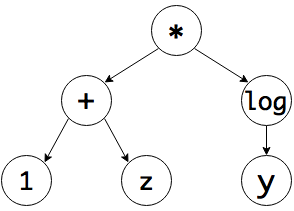
\includegraphics[width=4cm]{expr.png}
    \end{center}
  \item No need to store parentheses
  \item Each circle represents a \alert{node}
  \item A node has at most one parent and at most two children
  \end{itemize}
\end{frame}

\begin{frame}
  \frametitle{Expression trees (2/2)}
  \begin{itemize}
  \item In Dynare preprocessor, a tree node is a represented by an instance of the abstract class \texttt{ExprNode}
  \item This class has 5 sub-classes, corresponding to the 5 types of nodes:
    \begin{itemize}
    \item \texttt{NumConstNode} for constant nodes: contains the identifier of the numerical constants it represents
    \item \texttt{VariableNode} for variable/parameters nodes: contains the identifier of the variable or parameter it represents
    \item \texttt{UnaryOpNode} for unary operators (\textit{e.g.} unary minus, $\log$, $\sin$): contains an integer representing the operator, and a pointer to its child
    \item \texttt{BinaryOpNode} for binary operators (\textit{e.g.} $+$, $*$, pow): contains an integer representing the operator, and pointers to its two children
    \item \texttt{UnknownFunctionNode} for functions unknown to the parser (\textit{e.g.} user defined functions): contains the identifier of the function name, and a vector containing an arbitrary number of children (the function arguments)
    \end{itemize}
  \end{itemize}
\end{frame}

\begin{frame}
  \frametitle{Classes \texttt{DataTree} and \texttt{ModelTree}}
  \begin{itemize}
  \item Class \texttt{DataTree} is a container for storing a set of expression trees
  \item Class \texttt{ModelTree} is a sub-class of \texttt{DataTree}, specialized for storing a set of model equations (among other things, contains symbolic derivation algorithm)
  \item Class \texttt{ModFile} contains:
    \begin{itemize}
    \item one instance of \texttt{ModelTree} for storing the equations of model block
    \item one instance of \texttt{DataTree} for storing all expressions outside model block
    \end{itemize}
  \item Expression storage is optimized through three mechanisms:
    \begin{itemize}
    \item pre-computing of numerical constants
    \item symbolic simplification rules
    \item sub-expression sharing
    \end{itemize}
  \end{itemize}
\end{frame}

\begin{frame}
  \frametitle{Constructing expression trees}
  \begin{itemize}
  \item Class \texttt{DataTree} contains a set of methods for constructing expression trees
  \item Construction is done bottom-up, node by node:
    \begin{itemize}
    \item one method for adding a constant node (\texttt{AddPossiblyNegativeConstant(double)})
    \item one method for a log node (\texttt{AddLog(arg)})
    \item one method for a plus node (\texttt{AddPlus(arg1, arg2)})
    \end{itemize}
  \item These methods take pointers to \texttt{ExprNode}, allocate the memory for the node, construct it, and return its pointer
  \item These methods are called:
    \begin{itemize}
    \item from \texttt{ParsingDriver} in the semantic actions associated to the parsing of expressions
    \item during symbolic derivation, to create derivatives expressions
    \end{itemize}
  \item Note that \texttt{NodeID} is an alias (typedef) for \texttt{ExprNode*}
  \end{itemize}
\end{frame}

\begin{frame}
  \frametitle{Reduction of constants and symbolic simplifications}
  \begin{itemize}
  \item The construction methods compute constants whenever it is possible
    \begin{itemize}
    \item Suppose you ask to construct the node $1+1$
    \item The \texttt{AddPlus()} method will return a pointer to a constant node containing 2
    \end{itemize}
  \item The construction methods also apply a set of simplification rules, such as:
    \begin{itemize}
    \item $0+0=0$
    \item $x+0 = x$
    \item $0-x = -x$
    \item $-(-x) = x$
    \item $x*0 = 0$
    \item $x/1 = x$
    \item $x^0 = 1$
    \end{itemize}
  \item When a simplification rule applies, no new node is created
  \end{itemize}
\end{frame}

\begin{frame}
  \frametitle{Sub-expression sharing (1/2)}
  \begin{itemize}
  \item Consider the two following expressions: $(1+z)*\log(y)$ and $2^{(1+z)}$
  \item Expressions share a common sub-expression: $1+z$
  \item The internal representation of these expressions is:
    \begin{center}
      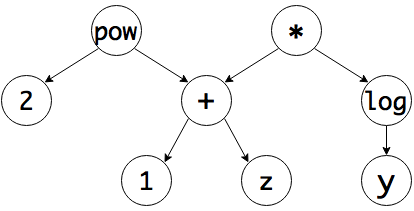
\includegraphics[width=6cm]{expr-sharing.png}
    \end{center}
  \end{itemize}
\end{frame}

\begin{frame}
  \frametitle{Sub-expression sharing (2/2)}
  \begin{itemize}
  \item Construction methods implement a simple algorithm which achieves maximal expression sharing
  \item Algorithm uses the fact that each node has a unique memory address (pointer to the corresponding instance of \texttt{ExprNode})
  \item It maintains 5 tables which keep track of the already constructed nodes: one table by type of node (constants, variables, unary ops, binary ops, unknown functions)
  \item Suppose you want to create the node $e_1+e_2$ (where $e_1$ and $e_2$ are sub-expressions):
    \begin{itemize}
    \item the algorithm searches the binary ops table for the tuple equal to (address of $e_1$, address of $e_2$, op code of +) (it is the \alert{search key})
    \item if the tuple is found in the table, the node already exists, and its memory address is returned
    \item otherwise, the node is created, and is added to the table with its search key
    \end{itemize}
  \item Maximum sharing is achieved, because expression trees are constructed bottom-up
  \end{itemize}
\end{frame}

\begin{frame}
  \frametitle{Final remarks about expressions}
  \begin{itemize}
  \item Storage of negative constants
    \begin{itemize}
    \item class \texttt{NumConstNode} only accepts positive constants
    \item a negative constant is stored as a unary minus applied to a positive constant
    \item this is a kind of identification constraint to avoid having two ways of representing negative constants: $(-2)$ and $-(2)$
    \end{itemize}
  \item Widely used constants
    \begin{itemize}
    \item class \texttt{DataTree} has attributes containing pointers to one, zero, and minus one constants
    \item these constants are used in many places (in simplification rules, in derivation algorithm...)
    \item sub-expression sharing algorithm ensures that those constants will never be duplicated
    \end{itemize}
  \end{itemize}
\end{frame}

\begin{frame}
  \frametitle{List of statements}
  \begin{itemize}
  \item A statement is represented by an instance of a subclass of the abstract class \texttt{Statement}
  \item Three groups of statements:
    \begin{itemize}
    \item initialization statements (parameter initialization with $p = \ldots$, \texttt{initval}, \texttt{histval} or \texttt{endval} block)
    \item shocks blocks
    \item computing tasks (\texttt{check}, \texttt{simul}, ...)
    \end{itemize}
  \item Each type of statement has its own class (\textit{e.g.} \texttt{InitValStatement}, \texttt{SimulStatement}, ...)
  \item The class \texttt{ModFile} stores a list of pointers of type \texttt{Statement*}, corresponding to the statements of the \texttt{mod} file, in their order of declaration
  \item Heavy use of polymorphism in the check pass, computing pass, and when writing outputs: abstract class \texttt{Statement} provides a virtual method for these 3 actions
  \end{itemize}
\end{frame}

\begin{frame}
  \frametitle{Evaluation context}
  \begin{itemize}
  \item The \texttt{ModFile} class contains an \alert{evaluation context}
  \item It is a map associating a numerical value to some symbols
  \item Filled in with \texttt{initval} block, and with parameters initializations
  \item Used during equation normalization (in the block decomposition), for finding non-zero entries in the jacobian
  \end{itemize}
\end{frame}

\section{Check pass}

\begin{frame}
  \frametitle{Error checking during parsing}
  \begin{itemize}
  \item Some errors in the \texttt{mod} file can be detected during the parsing:
    \begin{itemize}
    \item syntax errors
    \item use of undeclared symbol in model block, initval block...
    \item use of a symbol incompatible with its type (\textit{e.g.} parameter in initval, local variable used both in model and outside model)
    \item multiple shocks declaration for the same variable
    \end{itemize}
  \item But some other checks can only be done when parsing is completed
  \end{itemize}
\end{frame}

\begin{frame}
  \frametitle{Check pass}
  \begin{itemize}
  \item The check pass is implemented through method \texttt{ModFile::checkPass()}
  \item Does the following checks:
    \begin{itemize}
    \item check there is at least one equation in the model (except if doing a standalone BVAR estimation)
    \item check there is not both a \texttt{simul} and a \texttt{stoch\_simul} (or another command triggering local approximation)
    \end{itemize}
  \item Other checks could be added in the future, for example:
    \begin{itemize}
    \item check that every endogenous variable is used at least once in current period
    \item check there is a single \texttt{initval} (or \texttt{histval}, \texttt{endval}) block
    \item check that \texttt{varobs} is used if there is an estimation
    \end{itemize}
  \end{itemize}
\end{frame}

\section{Computing pass}

\begin{frame}
  \frametitle{Overview of the computing pass}
  \begin{itemize}
  \item Computing pass implemented in \texttt{ModFile::computingPass()}
  \item Begins with a determination of which derivatives to compute
  \item Then, calls \texttt{ModelTree::computingPass()}, which computes:
    \begin{itemize}
    \item leag/lag variable incidence matrix
    \item symbolic derivatives
    \item equation normalization + block decomposition (only in \texttt{sparse\_dll} mode)
    \item temporary terms
    \item symbolic gaussian elimination (only in \texttt{sparse\_dll} mode) \textit{(actually this is done in the output writing pass, but should be moved to the computing pass)}
    \end{itemize}
  \item Finally, calls \texttt{Statement::computingPass()} on all statements
  \end{itemize}
\end{frame}

\begin{frame}
  \frametitle{The variable table}
  \begin{itemize}
  \item In the context of class \texttt{ModelTree}, a \alert{variable} is a pair (symbol, lead/lag)
  \item The symbol must correspond to an endogenous or exogenous variable (in the sense of the model)
  \item The class \texttt{VariableTable} keeps track of those pairs
  \item An instance of \texttt{ModelTree} contains an instance of \texttt{VariableTable}
  \item Each pair (\texttt{symbol\_id}, lead/lag) is given a unique \texttt{variable\_id}
  \item After the computing pass, the class \texttt{VariableTable} writes the leag/lag incidence matrix:
    \begin{itemize}
    \item endogenous symbols in row
    \item leads/lags in column
    \item elements of the matrix are either 0 or correspond to a variable ID, depending on whether the pair (symbol, lead/lag) is used or not in the model
    \end{itemize}
  \end{itemize}
\end{frame}

\begin{frame}
  \frametitle{Static versus dynamic model}
  \begin{itemize}
  \item The static model is simply the (dynamic) model from which the leads/lags have been omitted
  \item Static model used to characterize the steady state
  \item The jacobian of the static model is used in the (Matlab) solver for determining the steady state
  \item No need to derive static and dynamic models independently: \\
    static derivatives can be easily deduced from dynamic derivatives
  \end{itemize}
  \begin{block}{Example}
    \begin{itemize}
    \item suppose dynamic model is $2x \cdot x_{-1} = 0$
    \item static model is $2x^2 = 0$, whose derivative w.r. to $x$ is $4x$
    \item dynamic derivative w.r. to $x$ is $2x_{-1}$, and w.r. to $x_{-1}$ is $2x$
    \item removing leads/lags from dynamic derivatives and summing over the two partial derivatives w.r. to $x$ and $x_{-1}$ gives $4x$
    \end{itemize}
  \end{block}
\end{frame}

\begin{frame}
  \frametitle{Which derivatives to compute ?}
  \begin{itemize}
  \item In deterministic mode:
    \begin{itemize}
    \item static jacobian (w.r. to endogenous variables only)
    \item dynamic jacobian (w.r. to endogenous variables only)
    \end{itemize}
  \item In stochastic mode:
    \begin{itemize}
    \item static jacobian (w.r. to endogenous variables only)
    \item dynamic jacobian (w.r. to all variables)
    \item possibly dynamic hessian (if \texttt{order} option $\geq 2$)
    \item possibly dynamic 3rd derivatives (if \texttt{order} option $\geq 3$)
    \end{itemize}
  \item For ramsey policy: the same as above, but with one further order of derivation than declared by the user with \texttt{order} option (the derivation order is determined in the check pass, see \texttt{RamseyPolicyStatement::checkPass()})
  \end{itemize}
\end{frame}

\begin{frame}
  \frametitle{Derivation algorithm (1/2)}
  \begin{itemize}
  \item Derivation of the model implemented in \texttt{ModelTree::derive()}
  \item Simply calls \texttt{ExprNode::getDerivative(varID)} on each equation node
  \item Use of polymorphism:
    \begin{itemize}
    \item for a constant or variable node, derivative is straightforward (0 or 1)
    \item for a unary or binary op node, recursively calls method \texttt{getDerivative()} on children to construct derivative of parent, using usual derivation rules, such as:
      \begin{itemize}
      \item $(log(e))' = \frac{e'}{e}$
      \item $(e_1 + e_2)' = e'_1 + e'_2$
      \item $(e_1 \cdot e_2)' = e'_1\cdot e_2 + e_1\cdot e'_2$
      \item $\ldots$
      \end{itemize}
    \end{itemize}
  \end{itemize}
\end{frame}

\begin{frame}
  \frametitle{Derivation algorithm (2/2)}
  \framesubtitle{Optimizations}
  \begin{itemize}
  \item Caching of derivation results
    \begin{itemize}
    \item method \texttt{ExprNode::getDerivative(varID)} memorizes its result in a member attribute the first time it is called
    \item so that the second time it is called (with the same argument), simply returns the cached value without recomputation
    \item caching is useful because of sub-expression sharing
    \end{itemize}
    \pause
  \item Symbolic \textit{a priori}
    \begin{itemize}
    \item consider the expression $x+y^2$
    \item without any computation, you know its derivative w.r. to $z$ is zero
    \item each node stores in an attribute the set of variables which appear in the expression it represents ($\{x,y\}$ in the example)
    \item that set is computed in the constructor (straigthforwardly for a variable or a constant, recursively for other nodes, using the sets of the children)
    \item when \texttt{getDerivative(varID)} is called, immediately returns zero if \texttt{varID} is not in that set
    \end{itemize}
  \end{itemize}
\end{frame}

\begin{frame}[fragile]
  \frametitle{Temporary terms (1/2)}
  \begin{itemize}
  \item When the preprocessor writes equations and derivatives in its outputs, it takes advantage of sub-expression sharing
  \item In Matlab static and dynamic output files, equations are preceded by a list of \alert{temporary terms}
  \item Those terms are temporary variables containing expressions shared by several equations or derivatives
  \item Doing so greatly enhances the computing speed of model residual, jacobian or hessian
  \end{itemize}
  \begin{block}{Example}
    \begin{columns}[t]
      \begin{column}{6cm}
        The equations:
\begin{verbatim}
residual(0)=x+y^2-z^3;
residual(1)=3*(x+y^2)+1;
\end{verbatim}
      \end{column}
      \begin{column}{4.8cm}
        Can be optimized in:
\begin{verbatim}
T01=x+y^2;
residual(0)=T01-z^3;
residual(1)=3*T01+1;
\end{verbatim}
      \end{column}
    \end{columns}
  \end{block}
\end{frame}

\begin{frame}
  \frametitle{Temporary terms (2/2)}
  \begin{itemize}
  \item Expression storage in the preprocessor implements maximal sharing...
  \item ...but it is not optimal for the Matlab output files, because creating a temporary variable also has a cost (in terms of CPU and of memory)
  \item Computation of temporary terms implements a trade-off between:
    \begin{itemize}
    \item cost of duplicating sub-expressions
    \item cost of creating new variables
    \end{itemize}
  \item Algorithm uses a recursive cost calculation, which marks some nodes as being ``temporary''
  \item \textit{Problem}: redundant with optimizations done by the C/C++ compiler (when Dynare is in DLL mode) $\Rightarrow$ compilation very slow on big models
  \end{itemize}
\end{frame}

\begin{frame}
  \frametitle{The special case of Ramsey policy}
  \begin{itemize}
  \item For most statements, the method \texttt{computingPass()} is a no-op...
  \item ...except for \texttt{planner\_objective} statement, which serves to declare planner objective when doing optimal policy under commitment
  \item Class \texttt{PlannerObjectiveStatement} contains an instance of \texttt{ModelTree}: used to store the objective (only one equation in the tree)
  \item During the computing pass, triggers the computation of the first and second order (static) derivatives of the objective
  \end{itemize}
\end{frame}

\section{Writing outputs}

\begin{frame}
  \frametitle{Output overview}
  \begin{itemize}
  \item Implemented in \texttt{ModFile::writeOutputFiles()}
  \item If \texttt{mod} file is \texttt{model.mod}, all created filenames will begin with \texttt{model}
  \item Main output file is \texttt{model.m}, containing:
    \begin{itemize}
    \item general initialization commands
    \item symbol table output (from \texttt{SymbolTable::writeOutput()})
    \item lead/lag incidence matrix (from \texttt{ModelTree::writeOutput()})
    \item call to Matlab functions corresponding to the statements of the \texttt{mod} file (written by calling \texttt{Statement::writeOutput()} on all statements through polymorphism)
    \end{itemize}
  \item Subsidiary output files:
    \begin{itemize}
    \item one for the static model
    \item one for the dynamic model
    \item and one for the planner objective (if relevant)
    \item written through \texttt{ModelTree} methods: \texttt{writeStaticFile()} and \texttt{writeDynamicFile()}
    \end{itemize}
  \end{itemize}
\end{frame}

\begin{frame}
  \frametitle{Model output files}
  Three possibles modes for \texttt{ModelTree} (see \texttt{mode} attribute):
  \begin{itemize}
  \item Standard mode: static and dynamic files in Matlab
  \item DLL mode:
    \begin{itemize}
    \item static and dynamic files in C++ source code (with corresponding headers)
    \item compiled through \texttt{mex} to allow execution from within Matlab
    \end{itemize}
  \item Sparse DLL mode:
    \begin{itemize}
    \item static file in Matlab
    \item two possibilities for dynamic file:
      \begin{itemize}
      \item by default, a C++ source file (with header) and a binary file, to be read from the C++ code
      \item or, with \texttt{no\_compiler} option, a binary file in custom format, executed from Matlab through \texttt{simulate} DLL
      \item the second option serves to bypass compilation of C++ file which can be very slow
      \end{itemize}
    \end{itemize}
  \end{itemize}
\end{frame}

\section{Conclusion}

\begin{frame}
  \frametitle{Future work (1/2)}
  \framesubtitle{Enhancements, optimizations}
  \begin{itemize}
  \item Refactor and reorganize some portions of the code
  \item Create a testsuite (with unitary tests)
  \item Separate computation of temporary terms between static and dynamic outputs
  \item Enhance sub-expression sharing algorithm (using associativity, commutativity and factorization rules)
  \item Add many checks on the structure of the \texttt{mod} file
  \end{itemize}
\end{frame}

\begin{frame}
  \frametitle{Future work (2/2)}
  \framesubtitle{Features}
  \begin{itemize}
  \item Add precompiler macros (\#include, \#define, \#if)
  \item Add handling for several (sub-)models
  \item Add indexed variables and control statements (if, loops) both in models and command language
  \item Add sum, diff, prod operators
  \item For unknown functions in the model: let user provide a derivative, or trigger numerical derivation
  \item Generalize binary code output
  \item Generalize block decomposition ?
  \end{itemize}
\end{frame}



\end{document}
